\chapter{Modifications to MAUT Based Generation of compound critiques}
\label{chap:modifications}
\section{Limitations of MAUT Based Critiquing:}

We have seen in Sections \ref{sec:offline} and \ref{sec:liveUser} that MAUT based recommendation performs slightly better than Apriori algorithm in offline experiments and live user studies.
However, there are several limitations to MAUT based recommendation, which when addressed can improve it's performance significantly.
The limitations to MAUT based recommendation are as follows:
\begin{itemize}
\setlength{\itemsep}{5pt}
\item Critique strings in a given iteration can be very similar to each other. This doesn't give the user too many options to choose from.
\item Preference model is updated only based on the most recently selected product. History of user selected products/critique strings is not considered while updating the preference model.
\item Top five products shown in the first cycle is same for all user-queries
\item In a particular recommendation cycle, if all the critique strings have "Higher Price", user is forced to select a critique string with "Higher Price". We would ideally not want to update the weight of the attribute $price$, since we cannot infer whether user is willing to compromise on $price$ attribute. But MAUT based recommendation algorithm will actually decrease the weight of $price$ attribute by a factor of $\beta$.
\item As an extension to the above point, Consider the case when there are 4 critique strings with "Lower Resolution" and 1 critique string with "Higher Resolution". If the user selects the critique string that has "Higher Resolution", we can update  the weight of 'Resolution' attribute by a higher factor.
\item The fact that a particular product has been preferred over the remaining (k-1) rejected products is not exploited

\end{itemize}
%put section numbers when all the description is done...
We try to address the above each of the above limitations in Sections (Numbers) and also propose some additional improvements that improve the performance of MAUT based recommendation.


\section{Diversity in Critiques}

A variant of \textit{\textbf{Bounded Greedy Selection}} algorithm described in \cite{boundedGreedy} was used to generate diverse critiques in every cycle.
The function \textit{GenCritiqueItems(PM, IS)} is modified as follows:\\
\\

\begin{algorithm}[ht]
  \SetKwInOut{Input}{input}\SetKwInOut{Output}{output}
  \DontPrintSemicolon
  %\Input{$PM$, $IS$}

  $R \gets \{\}$\\
  $CB' \gets IS$\\
  \For{ $i\gets0$ \KwTo $k$ }{
    Sort $CB'$ by $Quality(i, R, PM)$ for each case in IS; \\
    $R \gets R + First(CB')$;\\
    $CB' \gets CB' - First(CB')$;\\
  }
  \Return R
  \caption{GenCritiqueItems(PM, IS)}
  \label{algo:div}
\end{algorithm}

\begin{algorithm}[ht]
  \SetKwInOut{Input}{input}\SetKwInOut{Output}{output}
  \DontPrintSemicolon
  %\Input{$i$, $R$, $PM$}

  \If {$R == \{\}$} {return 0;}
  \Else {
      $retVal \gets \alpha \times utility(i, PM)$; \\
      $disSim \gets \frac{\sum_{r_j \in R} (1-critiqueSim(i,r_j))}{|R|}$;\\
      $retVal += (1-\alpha) \times disSim$;\\
      $return retVal$;\\
  }
  \Return retVal
  \caption{Quality(i, R, PM)}
  \label{algo:quality}
\end{algorithm}

$critiqueSim(a, b)$ returns the extent of overlap between the individual attribute directions of products $a$ and $b$.
We get the best results when $\alpha = 0.5$.
Introducing diverse critiques in every cycle results in significant improvement in the number of interaction cycles and it also improves user experience (Users don't prefer critiques being very similar to each other).


\begin{figure}
\centering
\begin{minipage}{.45\textwidth}
  \centering
  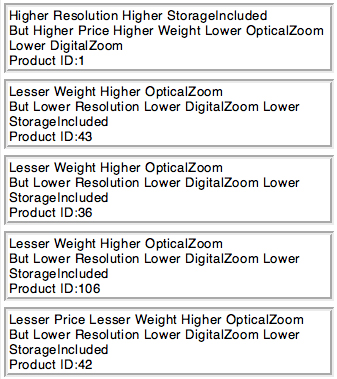
\includegraphics[width=1\linewidth]{figures-bharath/diversity1.jpg}
  \caption{Before diversifying critique strings}
  \label{fig:beforeDiv}
\end{minipage}%
\;\;\;\;\;\;
\begin{minipage}{.45\textwidth}
  \centering
  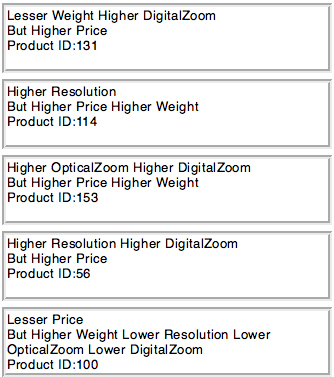
\includegraphics[width=1\linewidth]{figures-bharath/diversity2.jpg}
  \caption{After diversification}
  \label{fig:afterDiv}
\end{minipage}
\end{figure}



\section{Selectively updating value functions of nominal attributes}
As seen in Section \ref{sec:valueFunc}, the value of $\gamma$ used to update the value functions of nominal attributes is constant in each cycle.
Instead, we propose an alternative approach in which the value of $\gamma$ varies according to the number of alternatives the user rejected while choosing a particular attribute value. 
Stronger the preference the user has for a particular attribute value, higher is the value of $\gamma$.
The intuition for varying the value of $\gamma$ is as follows: Consider the case when there are five PCs displayed to the user and the manufacturers of the five PCs are "Compaq", "HP", "Apple", "Dell" and "Toshiba".
If the user selects the PC with "Compaq" as the manufacturer, we can see that he has accepted "Compaq" and rejected four other manufacturers.
Thus, we can say that the user has a strong preference for "Compaq" PCs.
On the other hand, in the case when all the five PCs have a screen size of 15 inches and the user selects the PC with screen-size of 15 inches, we cannot really infer whether the user has a strong preference for 15 inch PCs.
Generalizing the examples above, if $k$ is the value of the attribute N selected in a cycle and $R$ is the list of values of attribute $N$ of the top-K products other than the selected products, we define
%
\begin{equation}
\gamma = \frac{\#\: of\: alternatives\: to\: k\: in\: R}{|R|}
\end{equation}
%
If attribute $N$ = "Manufacturer"; $\gamma$ = 1 when manufacturer of all the remaining products is different from the selected product's manufacturer($M$) and also different from each other; meaning that the user has a strong preference for $M$.
$\gamma$ = 0 when manufacturer of all remaining products is same as the selected product's manufacturer($M$).
This is the case when we cannot infer whether the user has a strong preference for $M$.
This is similar to weighted MLT described in \cite{comparisonbr}.
Some examples of how the value of $\gamma$ varies are illustrated in Table \ref{tab:wMLT}
Varying the value of $\gamma$ according to the other products' attribute values results in a significant improvement in the number of interaction cycles.



\begin{table}
\renewcommand{\arraystretch}{1.5}
 \centering
 \begin{tabular}{l l l l l l |l|}
  \hline \hline
   Feature & P1 & P2 & P3 & P4 & P5 & $\gamma$ \\
  \hline
  Manufacturer & Dell & Apple & Compaq & HP & Toshiba & 1.0 \\
  Type & Laptop & Laptop & Laptop & Laptop & Laptop & 0 \\
  Processor & Core-i3 & AMD-E1 & Core-i7 & AMD-E1 & Core-i3 & 0.5\\
  Screen-size & 15 & 13.3 & 15 & 15 & 15 & 0.25\\
  \hline \hline
 \end{tabular}
 \caption{Values of $\gamma$ when P3 is selected by the user}
 \label{tab:wMLT}
\end{table}


\section{Additional preference to products that are similar to the most recent user selected product}
In addition to updating weights of numeric attributes and value functions of nominal attributes, we give an additional preference to the products that have a similar critique pattern as that of the most recently selected product.
The method of computing critique patterns for products has been discussed in Section \ref{sec:genCritique}.
The intuition behind this modification is that, if the user selects the critique string "Lower Price, Higher Resolution but Higher Weight", he is interested in those products where this trade-off is obeyed.
Considering only three attributes, Price, Resolution and Weight, if the critique pattern of the selected product is \{Price:$<$, Resolution:$>$, Weight:$>$\} and the critique pattern of a product $p$ in the case base is \{Price:$<$, Resolution:$>$, Weight:$<$\}, the overlap between the two critique patterns is 2/3.
The function $CalcUtility(PM, u)$ (Algorithm \ref{algo:utility}), which is used to calculate utility of products at the beginning of each cycle is modified as follows:

\begin{algorithm}[ht]
  \SetKwInOut{Input}{input}\SetKwInOut{Output}{output}
  \DontPrintSemicolon
  %\Input{$PM$, $IS$}

  retVal $\gets 0$;\\
  \For{ each attribute $x_i$ in $u$ }{
      retVal += $pw_i \times V(x_i)$
  }
  $p1 \gets $CritiquePattern(u);\\
  $p2 \gets $CritiquePattern(previousSelectedProduct);\\
  retVal += $overlap(p1, p2)$;\\
  \Return retVal
  \caption{CalcUtility(PM, u)}
  \label{algo:addPref}
\end{algorithm}



%\subsection{Generalization of the above where you can have multiple products}
In Algorithm \ref{algo:addPref}, we have considered the critique overlap between a product in the case-base and the product that is most recently selected by the user.
We now extend the above algorithm by considering the critique overlap of a product with all the products that have been selected so far.
The additional term added to the utility of a product,\textit{overlapTerm} is calculated as follows:
\begin{equation}
\label{eq:addPref}
addTerm(p) = \frac{\sum_{i=1}^{n} {w_i \times overlap(p,sel_i)}} {\sum_{i=1}^{n}w_i}
\end{equation}
In Equation \ref{eq:addPref}, $sel_i$ refers to the product selected by the user in $i^{th}$ cycle.
$w_i$ is the weight/importance associated with the overlap between the product $p$ and product selected in $i^{th}$ cycle.
In our implementation, we set $w_i = \frac{1}{2^{n-i}}$.
The modified \textit{CalcUtility(PM, u)} function is as follows:

\begin{algorithm}[ht]
  \SetKwInOut{Input}{input}\SetKwInOut{Output}{output}
  \DontPrintSemicolon
  %\Input{$PM$, $IS$}

  retVal $\gets 0$;\\
  \For{ each attribute $x_i$ in $u$ }{
      retVal += $pw_i \times V(x_i)$
  }
  \For { each product $t_i$ in previouslySelectedProducts} {
      $p1 \gets $CritiquePattern($u$);\\
      $p2 \gets $CritiquePattern($t_i$);\\
      retVal += $w_i \times overlap(p1, p2)$;\\
  }
  \Return retVal
  \caption{CalcUtility(PM, u)}
  \label{algo:addPref2}
\end{algorithm}

\section{Varying the level of diversity}
\label{sec:div2}
In Section \ref{sec:div}, we have discussed a method of introducing diversity in every cycle.
We know that, at the beginning of a recommendation session, an average user does not have a good understanding of the product space and trade-offs that exist between different product attributes.
But after interacting with the recommender system for a few cycles, he develops a good understanding of the product space and his preferences become more stable.
Therefore, it is a good idea to introduce diversity in the beginning of a recommendation session so that user will develop a better understanding of the product space and then show targeted recommendations after a few cycles when his preferences have stabilized.

We propose a new approach where diversity is varied adaptively according to whether user's preferences have stabilized.
Consider an attribute 'Price'.
If the maximum difference between prices of previous $K$(=3) products selected by the user is less than a pre-defined threshold, we assume that the user is satisfied with this particular product price and we promote cases that have a price closer to the average price of the $K$ products in the next cycle.
%Consdiering camera dataset, if the difference between 'weight' of each of the previous $K$(=3) selected products is less than a certain threshold,
If the maximum difference between the weights of the previous $K$(=3) products is greater than the pre-defined threshold, we assume that user's preference for the 'weight' attribute has not stabilized yet. 
Hence, we try to display products that are diverse to each other in terms of 'weight' attribute.
The numeric attributes for which we assume that user's preference has stabilized are classified into the set $simA$.
The other numeric attributes are classified into the set $divA$.
In the implementation, the function \textit{GenCritiqueItems(PM, IS)} is the same as described in Algorithm \ref{algo:div}.
The function \textit{Quality(p, R, PM)} is modified as follows:

\begin{algorithm}[ht]
  \SetKwInOut{Input}{input}\SetKwInOut{Output}{output}
  \DontPrintSemicolon
  %\Input{$i$, $R$, $PM$}

  $ret \gets \alpha \times utility(i, PM)$; \\
  $simA, divA$ = classifyAttributes(); \\
  $avg$ = previousKProductAttributeAverages(); \\
  $tmp \gets 0$;\\
  \For{ each attribute $x_i$ in $simA$ }{
      $tmp$ += (sim($avg(x_i)$, $p(x_i)$));\\
  }
  \For{ each attribute $x_i$ in $divA$ }{
      $tmp += \frac{\sum_{r_j \in R} (1-sim(p(x_i),r_j(x_i)))}{|R|}$;\\
  }

  $tmp = (1-\alpha) \times \frac{tmp} {\lvert simA\rvert + \lvert divA\rvert}$\\
  \Return $ret + tmp$ ;\\
  \caption{Quality(p, R, PM)}
  \label{algo:quality2}
\end{algorithm}

We will refer to the algorithm described in this section as \textbf{DIV2} in the subsequent sections.



